\documentclass[11pt]{article}

% Review version for EMNLP 2026 / ARR-style submission.
% Switch to \usepackage{acl} for the camera-ready version.
\usepackage[review]{acl}

\usepackage{times}
\usepackage{latexsym}
\usepackage[T1]{fontenc}
\usepackage[utf8]{inputenc}
\usepackage{microtype}
\usepackage{inconsolata}
\usepackage{graphicx}
\usepackage{booktabs}
\usepackage{amsmath}

\title{ChronoStream: Agentic Temporal Reasoning for Streaming Video Understanding}

\author{Anonymous EMNLP 2026 Submission}

\begin{document}
\maketitle

\begin{abstract}
Real-time video understanding requires models to reason while a stream is still unfolding, rather than after the full video has been observed.
We introduce ChronoStream, an agentic temporal reasoning framework for streaming video understanding.
ChronoStream maintains a bounded, source-linked temporal memory, consolidates observed intervals into compact summaries, and recalls time-anchored history when a query requires past evidence.
TODO: Replace this placeholder with the final 200-word abstract after main experiments are frozen.
\end{abstract}

\section{Introduction}

Video large language models have substantially advanced video question answering, long-video understanding, and temporal localization \citep{mvbench2024,longvideobench2024,videomme2025}.
Most of these settings, however, assume that a complete video is available before answering.
Streaming video understanding removes this assumption: visual observations arrive over time, user queries may appear at arbitrary moments, and the evidence required for an answer may lie before the query, at the query time, or only become visible afterwards.
Benchmarks such as StreamingBench and OVO-Bench make this distinction explicit by evaluating real-time understanding, backward tracing, and forward active responding under timestamped interaction \citep{streamingbench2024,ovobench2025}.
Thus, a streaming model must maintain an evolving temporal understanding using only the video that has arrived so far, while operating under bounded context and real-time response constraints.

To make video models operate online, existing methods mainly form two paradigms.
Response-control methods use output states or readiness prediction to let the model decide, during continuous observation, whether the current information is sufficient for answering \citep{videollm_online2024,livecc2025,streamready2026,streamo2026,aura2026}.
State-maintenance methods use cache windows or hierarchical memory to fold the growing video history into a fixed budget, keeping long-stream reasoning computationally feasible \citep{streamingvlm2025,fluxmem2026,streamforest2025,thinkstream2026,vst2026}.
These methods improve response timing and context scale, respectively, but they usually treat history as a state written forward over time.
If an early video segment only becomes necessary after a later query appears, the model lacks a mechanism to recall, reorganize, and use that segment with temporal anchors.

We argue that strong streaming video understanding requires \emph{thinking with time}: treating temporal history not as passive context, but as an actionable reasoning substrate.
First, a model should maintain long-horizon memory under a fixed budget rather than rely on an ever-growing visual context.
Second, it should consolidate observed intervals into compact summaries while preserving their temporal sources.
Third, it should be able to recall time-anchored history when the current query requires earlier evidence.
This view is aligned with recent agentic multimodal reasoning, where models learn to actively acquire and integrate evidence during reasoning \citep{deepeyes2026,deepeyesv22026}, and with long-context memory agents that replace unbounded input with learned memory updates and recallable memory states \citep{memagent2025,rememr12026}.

We introduce \textbf{ChronoStream}, an agentic temporal reasoning framework for streaming video understanding.
ChronoStream extends a forward streaming state into a recallable temporal memory and uses a single chunk-wise agent trajectory to coordinate current observation, memory consolidation, time-anchored recall, and answer generation.
At each step, the model updates its understanding from the current visual window, temporal memory, and pending queries.
When the current state is insufficient, it can issue a recall over a specified time range; when the memory reaches its budget, selected intervals are consolidated into source-linked summaries; when sufficient temporal evidence is available, the model emits an answer to the query.
This loop turns long-term memory from a passive cache into an internal state that the model can maintain, recall, and use for streaming reasoning.

Our contributions are as follows.
First, we formulate streaming video understanding as agentic temporal reasoning, shifting the focus from only deciding when to answer to deciding how to manage temporal evidence before answering.
Second, we propose ChronoStream, a streaming video agent that maintains bounded, source-linked, and time-recallable memory beyond the current visual window.
Third, we provide a unified chunk-wise agent trajectory that places interval consolidation, time-anchored recall, and query answering in the same generation process.
TODO: Add final empirical contribution once OVO-Bench, StreamingBench, and efficiency results are frozen.

\begin{figure}[t]
  \centering
  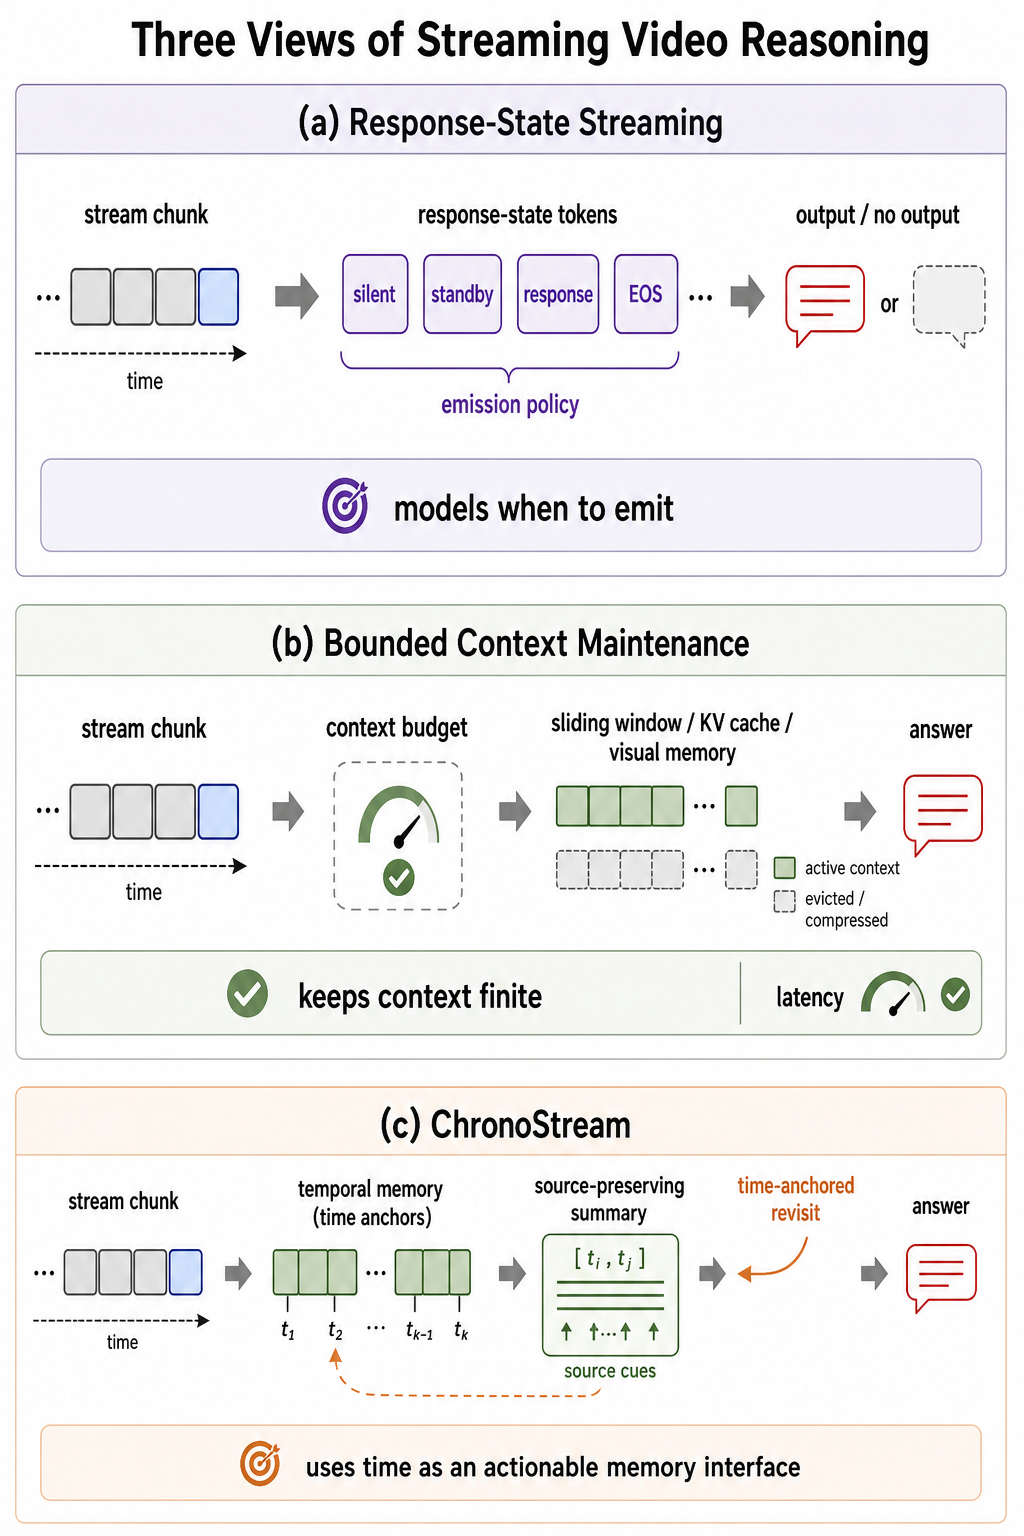
\includegraphics[width=\columnwidth]{../figures/chronostream_fig1_singlecol_v3_components.png}
  \caption{Motivation and method comparison for ChronoStream. Response-state streaming learns when to emit silent or response tokens, while streaming context management controls cost through windows, cache compression, or clustered memory. ChronoStream instead maintains bounded, source-linked temporal memory and can recall time-anchored history before answering.}
  \label{fig:chronostream-motivation}
\end{figure}

\section{Related Work}

\paragraph{VideoLLMs and streaming video understanding.}
Recent VideoLLMs and benchmarks have expanded video understanding from short clips to long, temporally structured videos \citep{mvbench2024,longvideobench2024,videomme2025}.
StreamingBench and OVO-Bench further highlight that online video understanding requires timestamp-aware interaction rather than post hoc reasoning over a complete video \citep{streamingbench2024,ovobench2025}.
Streaming systems such as VideoLLM-online, LiveCC, StreamReady, Streamo, and AURA model real-time output through streaming EOS, readiness prediction, response-state tokens, or unified always-on interaction \citep{videollm_online2024,livecc2025,streamready2026,streamo2026,aura2026}.
ChronoStream follows this online setting, but focuses on how temporal memory is maintained and recalled before an answer is produced.

\paragraph{Streaming context and memory management.}
Long-running streams require the model to keep history under bounded context, memory, and latency budgets.
StreamingVLM and related cache methods maintain compact KV states for infinite or long video streams \citep{streamingvlm2025}.
FluxMem and StreamForest organize history through adaptive hierarchical visual memory or persistent event memory \citep{fluxmem2026,streamforest2025}.
ThinkStream and VST convert observed video or intermediate reasoning into textual semantic memory to reduce response latency after the query \citep{thinkstream2026,vst2026}.
These methods make streaming computation affordable, while ChronoStream emphasizes a complementary capability: time-anchored recall over source-linked memory when a later query requires past evidence.

\paragraph{Agentic reasoning with tools and memory.}
Agentic multimodal reasoning methods place evidence acquisition inside the model's reasoning trajectory.
DeepEyes learns to ``think with images'' through active visual operations, while DeepEyesV2 extends this idea to general tool invocation with code execution and search \citep{deepeyes2026,deepeyesv22026}.
In long-context language reasoning, MemAgent reads long documents as sequential chunks and updates a fixed-length memory, while ReMemR1 augments this paradigm with callback-based memory retrieval so the model can learn when and what to recall \citep{memagent2025,rememr12026}.
ChronoStream brings this evidence-operation view into streaming video, where evidence is time-indexed, queries arrive asynchronously, and memory operations must remain compatible with online causality.

\section{Task Formulation}

TODO: Define streaming observations, per-timestep queries, action space, memory state, and evaluation protocol.

\section{Method}

\subsection{Watch-Think-Speak}

TODO: Describe the agent loop and the four action types: silent, response, recall, and compress.

\subsection{Reasoning-Compressed Streaming Memory}

TODO: Explain recent thoughts, compressed summaries, recall, and token budget control.

\subsection{Training}

TODO: Describe SFT, streaming RLVR / GDPO, reward components, and training-inference consistency.

\section{Experiments}

\subsection{Benchmarks}

We evaluate on the original OVO-Bench annotations rather than the probe-expanded single-question format.
For ChronoStream, each sample is executed as a full video trajectory: the agent starts from the beginning of the video, receives chunks in temporal order, maintains its memory state, optionally recalls past evidence, and answers only from observations that have arrived so far.
This protocol is used for real-time and backward-tracing tasks as well as forward active responding tasks such as REC, SSR, and CRR, where each probe is scored at its annotated time.

For base VideoLLM comparisons, we report both streaming and offline settings.
The streaming base receives uniformly sampled frames from the same recent temporal window available to the agent at the probe time.
The offline base receives uniformly sampled frames from the entire causal prefix from the start of the video to the probe or question time, never from the future.
This offline setting is intentionally a strong baseline rather than a weakened one: it gives the base model global access to all visual evidence that has appeared so far, without requiring it to compress memory or decide when to recall.
It therefore measures the underlying video understanding capacity of a plain VideoLLM under a generous causal context budget.
ChronoStream is more constrained in raw visual access, because it operates with a fixed current window and bounded textual memory, but is allowed to maintain, consolidate, and recall temporal evidence throughout the stream.
We report content accuracy together with timing-aware variants that separately count correct early, late, and exactly-on-probe responses, so gains cannot be explained by answering at an incorrect time.

\subsection{Main Results}

TODO: Insert main comparison table.

\subsection{Ablations}

TODO: Memory, recall, compression, RL reward, and sliding-window ablations.

\subsection{Efficiency}

TODO: Report latency, memory, and sequence length behavior under increasing video duration.

\section{Analysis}

TODO: Add qualitative examples, failure modes, and timing behavior.

\section{Conclusion}

TODO: Summarize contributions and future work.

\section*{Limitations}

TODO: Required by ACL/EMNLP style. Discuss limitations without adding new experiments, figures, or analysis.

\section*{Ethical Considerations}

TODO: Discuss data, privacy, misuse, and deployment risks for streaming video agents.

\bibliography{references}

\appendix

\section{Implementation Details}

TODO: Add dataset construction, prompts, reward details, and hyperparameters that do not fit in the main paper.

\end{document}
